\section{Thermal noise in resistor}

This section will issue the problem of thermal noise in resistors based on three different circuit topologies, which are:

\begin{itemize}
    \item Single noisy resistor;
    \item Noisy resistor associated with an ideal resistor;
    \item Noisy resistor associated with an ideal capacitor;
\end{itemize}

\subsection{Single noisy resistor}

First of all the spot noise for a resistor of $R = 50 \Omega$ at $T = 300K$ ($26.85^{\circ}$) is computed to serve as a theoretical basis. Therefore the noise power spectral density (PSD) is computed with the equation \ref{eq:spotnoise} ($k = 1.38064852 \times 10^{23} \, m^2 \, kg \, s^{-2} \, K^{-1}$ it is the Boltzmann constant):

\begin{equation} \label{eq:spotnoise}
    S_n(f) = 4 k T R = 8.28 \times 10^{-19} \, V^2/Hz
\end{equation}

So a transient simulation was executed for $1 ms$ of duration with a max. time step of $1 ns$. The temperature whose the resistor will operate was carefully set in the transient simulation options. The circuit setup follows the schematic of figure \ref{ckt:1} so the noise voltage can be correctly measured.


\begin{figure}[H]
\centering

\tikz \node [scale=0.8, inner sep=0] {
\begin{tikzpicture} [american]
    \draw[>=triangle 90, ->] (6.5,0) -- (5.5,0);
    \node[black] at (7,0) {$V_{noise}$}; 
    \draw (1,0) to[R, l=$R$, -*] (5,0)
    (1,0) -- (1,-0.2) node[ground]{}
    ;
\end{tikzpicture}
};

\caption{Circuit setup to measure single noisy resistor voltage. Source: own.}
\label{ckt:1} 
\end{figure}

The figure \ref{fig:trans1} leads one to think that the noise has a high amplitude. But zooming in the plot to a shorter time range like in figure \ref{fig:trans1}b, the low amplitude noise prevails and the high amplitude noise come to be only artifacts that appears sporadically.

\begin{figure}[H] 
\centering
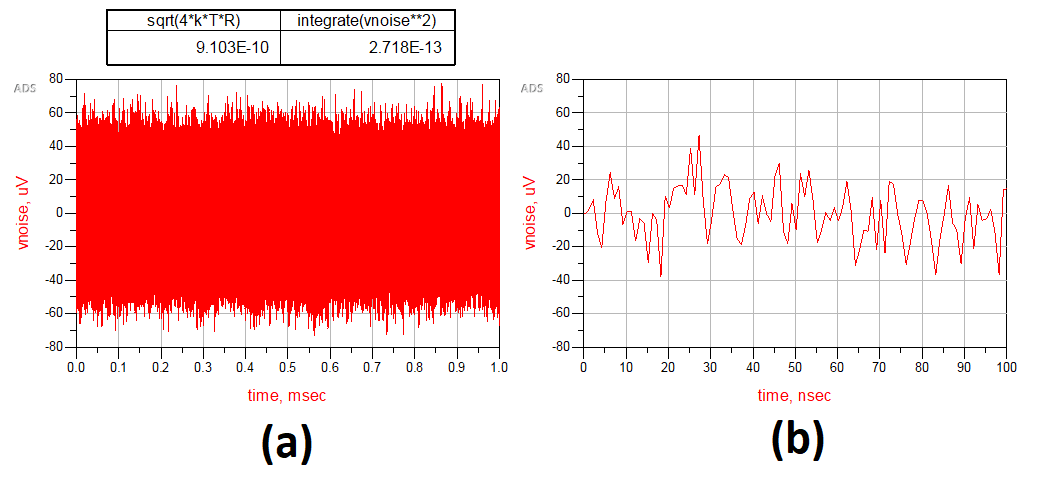
\includegraphics[width=13cm]{images/vnoise_trans.png}
\caption{Noise voltage in the terminal of a single resistor.}
\label{fig:trans1} 
\end{figure}

In practice the values of noise power spectral density for a transient simulation in figure \ref{fig:trans1} does not match the theoretical one. This is explained by the inherent limitations of transient simulation. 

Once the maximum time step was set to $1ns$, according to the Nyquist criterion, the highest frequency that can be reproduced in this simulation is equal to $f_N = \frac{1}{1 \times 10^{-9}} \times \frac{1}{2} = 500 MHz$. Once the theoretical value takes into account the whole infinity spectrum, the simulation is limited to a small portion of it. Reducing the max. time step will improve results, but it will take too much time to simulate. A simpler solution is to perform an AC simulation, varying frequency instead of time.

Now with a AC simulation varying the frequency from 1 Hz to 100 GHz and same topology as figure \ref{ckt:1}, we may observe in figure \ref{fig:ac1} that the practical spot noise match the PSD theoretical value for both cases of $R = 50\Omega$ and $R= 200 \Omega$. Also it prove that the PSD rises proportional to the resistance.

\begin{figure}[H] 
\centering
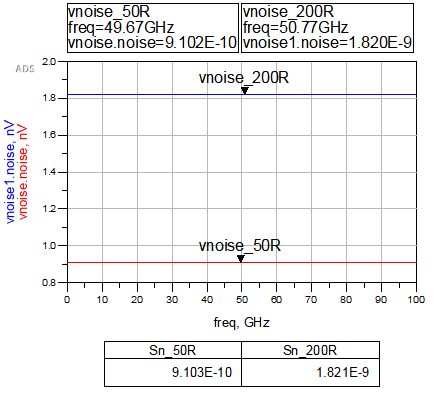
\includegraphics[width=10cm]{images/vnoise_ac.png}
\caption{Noise PSD for single resistor in two resistance conditions: $50 \Omega$ and $200 \Omega$.}
\label{fig:ac1} 
\end{figure}


\subsection{Noisy resistor associated with an ideal resistor}

From now on the transient simulation will not be used since the AC simulation show better results.

This section will work with a different circuit topology. As we can see in the schematic of figure \ref{ckt:2} the circuit consists of two combined resistors, but only one generate thermal noise.

\begin{figure}[H]
\centering

\tikz \node [scale=0.95, inner sep=0] {
\begin{tikzpicture} [american]
    \draw (0,0) -- (0,3)
    (0,3) to[generic, l=$Z_{2th}$] (3,3)
    (3,3) to[generic, l=$Z_{2trafo}$] (6,3)
    (5.5,3) to[short, l=$I_2$, i=$ $] (7,3) 
    (0,0) -- (7,0)
    (3,2.5) -- (3,3.5) 
    (7,2.5) -- (7,3.5);
    \node[black] at (3,3.8) {PE};
    \node[black] at (7,3.8) {BT};
\end{tikzpicture}
};

\caption{Circuito de sequência negativa do sistema proposto.}
\label{ckt:2} 
\end{figure}

According to the theory, considering the load resistor $R_L$ without noise and the other $R_T$ a resistor with noise, the expression for the available noise power density in given by \ref{eq:Rcomb}. Considering both resistors to be equal $R = R_L = R_T$, the expression \ref{eq:Rcomb} becomes independent of the resistor value and depend only on the temperature.

\begin{equation} \label{eq:Rcomb}
    \overline{v_{n,out}^2} = 4kT \left(\frac{R_L}{R_L+R_T} \right)^2 =  4kT \left(\frac{R}{2R} \right)^2 = kT
\end{equation}

Simulating the circuit for $R=R_L=R_T= 200 \Omega$ (and after for $500 \Omega$ and $1000 \Omega$), the available noise power density becomes $\overline{v_{n,out}^2} = 1.38064852 \times 10^{23} \times 300 = 4.143 \times 10^{-21} V^2/Hz$. In practice, the figure \ref{fig:ac2} show the results for an AC simulation with same parameters as before,  

\begin{figure}[H] 
\centering
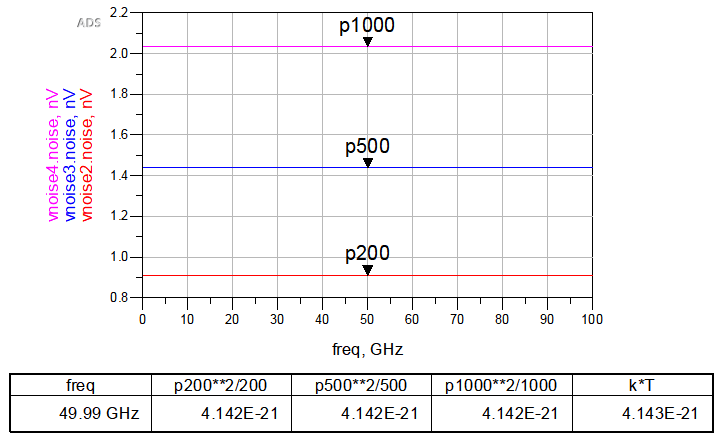
\includegraphics[width=10cm]{images/pnoise.png}
\caption{Noise PSD for combination of equal resistance resistors, but one noise and the other not in three resistance conditions: $200 \Omega$, $500 \Omega$ and $1000 \Omega$.}
\label{fig:ac2} 
\end{figure}

Since the noise power density is non dependent on the resistance value (at least the resistors must to have the same resistance), we observe in the figure \ref{fig:ac2} that all the three circuits show the same noise level which is equal to the theoretical value.


\subsection{Noisy resistor associated with an ideal capacitor}

In this section the topology of the circuit to measure noise is as follows in the figure \ref{ckt:3}.


\begin{figure}[H]
\centering

\tikz \node [scale=0.8, inner sep=0] {
\begin{tikzpicture} [american]
    \draw[>=triangle 90, ->] (6.5,0) -- (5.5,0);
    \node[black] at (7,0) {$V_{noise}$}; 
    \draw  (4,0) to[R, l=$C$, *-] (4,-4) node[ground]{}
    (2,0) to[R, l=$R$, -] (2,-4) node[ground]{}
    (2,0) -- (5,0)
    ;
\end{tikzpicture}
};

\caption{Circuit setup to measure noisy resistor voltage in a RC circuit with a ideal capacitor. Source: own.}
\label{ckt:3} 
\end{figure}

In this case the total power must be $\overline{v_{n,out}^2} = \frac{kT}{C}$, so it is expected that the noise power drops with a risen capacitance and keeps the same with a varying resistance. 

Simulating for $C=100pF$ and the resistors varying from $50 \Omega$, $200 \Omega$ and $1 k\Omega$, the plot of figure \ref{fig:ac3} is obtained.

\begin{figure}[H] 
\centering
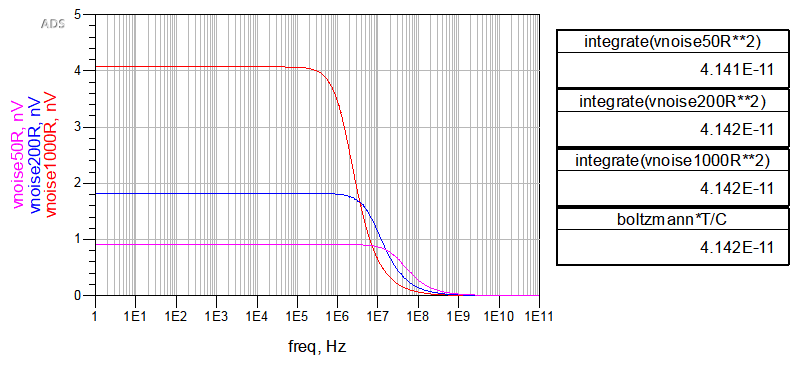
\includegraphics[width=12cm]{images/rcnoise.png}
\caption{Noise voltage behaviour and total noise power for a RC circuit topology and three resistance conditions: $50 \Omega$, $200 \Omega$ and $1 k\Omega$.}
\label{fig:ac3} 
\end{figure}

The theoretical value for the total noise power is computed in the figure \ref{fig:ac3} along side of the practical results, and once they are equal, it became proved that the total noise power in this circuit topology is non dependent on the resistance value.

A curious fact is the noise voltage behaviour. In the pure R circuit the noise voltage kept constant along all frequencies, but in the case of a RC circuit the noise in higher frequencies is filtered due to the capacitor. In this case the circuit by itself get rid of the noise in higher frequencies, no needing any design intervention.